%
% Parameters
%

\ifdefined\fullversion
\else
\def\fullversion{1}    % 0 = conference version; 1 = full version
\fi

\ifdefined\cameraversion
\else
\def\cameraversion{0}    % 0 = long version; 1 = proceedings version
\fi

\def\showoverflow{1}   % 1 = show overflows
\def\allow{1}      % 0 = remove todo command
\def\anonymous{0}      % 1 = anonymous

%
% Document class 
%

\documentclass[envcountsame,runningheads,notitlepage]{llncs}
\ifnum\fullversion=1
\usepackage[a4paper, margin=1.1in]{geometry}
\setlength{\marginparwidth}{2.5cm}
\fi

%
% Custom header
%

%!TEX root=../main.tex

% Packages
%

\usepackage[utf8]{inputenc}
\usepackage[T1]{fontenc}
\usepackage{hyperref}
\usepackage{verbatim}
\usepackage{tikz}
\usetikzlibrary{positioning,calc}
\usepackage{xspace}
\usepackage{amsmath} %\usepackage{amsthm}
\usepackage{amssymb}
\usepackage{mathtools}
\usepackage{pifont}
\usepackage{etoolbox}
\usepackage[normalem]{ulem}
\usepackage{booktabs}
\usepackage{array}
\usepackage[capitalise,noabbrev]{cleveref}
\usepackage{cite}
\usepackage{multibib}
\usepackage{url}
\usepackage{algorithm}
\usepackage{algpseudocode}
\usepackage{paralist}
\usepackage{mathrsfs}
\usepackage{relsize}
\usepackage{stmaryrd}
\usepackage[textsize=small]{todonotes}
\usepackage{multirow}
\usepackage[lambda,n,operators]{cryptocode}

\newtoggle{notes}
\toggletrue{notes} % set to false to remove colored notes from the paper

%--------------------------------------------------------
% Editorial
%--------------------------------------------------------

\newcommand{\redunderline}[1]{\textcolor{red}{\underline{\textcolor{black}{#1}}}} 
\newcommand{\TBW}{\textcolor{blue}{\textbf{To Be Written...}}}
\newcommand{\Note}[1]{\textcolor{magenta}{ $\langle \! \langle$ #1 $\rangle \! \rangle$}}
\newcommand{\todonote}[1]{\todo[inline]{MyName: #1}}

%--------------------------------------------------------
% General notations
%--------------------------------------------------------

\let\vec\mathbf
\newcommand{\bit}{\ensuremath{\{0,1\}}\xspace}
\newcommand{\getsr}{\leftarrow_{r}}
\newcommand{\poly}{\ensuremath{\mathsf{poly}}\xspace}

%--------------------------------------------------------
% Standard proba, games, proofs, sampling, distributions
%--------------------------------------------------------

\newcommand{\Good}{\ensuremath{\mathsf{Good}}\xspace}
\newcommand{\Bad}{\ensuremath{\mathsf{Bad}}\xspace}
\newcommand{\equivStat}{\ensuremath{\overset{\mathsf{stat}}{\equiv}}\xspace}
\newcommand{\equivComp}{\ensuremath{\overset{\mathsf{comp}}{\equiv}}\xspace}
\newcommand{\view}{\ensuremath{\textsc{View}}\xspace}
\newcommand{\state}{\ensuremath{\mathsf{st}}\xspace}
\newcommand{\st}{\state}
\newcommand{\Hyb}{\ensuremath{\mathsf{Hyb}}\xspace}
\newcommand{\Exp}{\ensuremath{\mathsf{Exp}}\xspace}
\newcommand{\myGame}{\ensuremath{\mathsf{Game}}\xspace}
\newcommand{\Event}{\ensuremath{\mathsf{E}}\xspace}
\newcommand{\Span}{\ensuremath{\mathsf{Span}}}
\newcommand{\prob}[1]{{\Pr}\left[\,{#1}\,\right]}
\newcommand{\probb}[2]{{\Pr}_{#1}\left[\,{#2}\,\right]}
\newcommand{\Dx}{\mathcal{D}}
\newcommand{\Hx}{\mathcal{H}}
\newcommand{\Sx}{\mathcal{S}}
\newcommand{\Lx}{\mathcal{L}}
\newcommand{\Dist}{\mathcal{D}}
\newcommand{\Expect}{\ensuremath{\mathbb{E}}\xspace}
\newcommand{\Sample}{\ensuremath{\mathsf{Sample}}\xspace}
\newcommand{\Sim}{\ensuremath{\mathsf{Sim}}\xspace}

%--------------------------------------------------------
% Adversaries, oracles
%--------------------------------------------------------

\newcommand{\AdvA}{\ensuremath{\mathcal{A}}\xspace}
\newcommand{\AdvB}{\ensuremath{\mathcal{B}}\xspace}
\newcommand{\AdvC}{\ensuremath{\mathcal{C}}\xspace}
\newcommand{\AdvD}{\ensuremath{\mathcal{D}}\xspace}

\newcommand{\adv}{\ensuremath{\mathsf{Adv}}\xspace}
\newcommand{\oracle}{\ensuremath{\mathcal{O}}\xspace}

%--------------------------------------------------------
% Classes, sets, groups
%--------------------------------------------------------

\newcommand{\BPP}{\ensuremath{\mathsf{BPP}}\xspace}
\newcommand{\NP}{\ensuremath{\mathsf{NP}}\xspace}
\newcommand{\coNP}{\ensuremath{\mathsf{coNP}}\xspace}
\newcommand{\PSPACE}{\ensuremath{\mathsf{PSPACE}}\xspace}
\newcommand{\NC}{\ensuremath{\mathsf{NC}}\xspace}

\newcommand{\Z}{\mathbb{Z}}
\newcommand{\F}{\mathbb{F}}
\newcommand{\N}{\mathbb{N}}
\newcommand{\R}{\mathbb{R}}
\newcommand{\G}{\mathbb{G}}
\newcommand{\Gt}{\mathbb{G}_{\mathsf{T}}}
\newcommand{\Hset}{\mathbb{H}}
\newcommand{\Zn}{\mathbb{Z}_n}
\newcommand{\Group}{\mathbb{G}}

\newcommand{\Lang}{\ensuremath{\mathscr{L}}}
\newcommand{\Lpar}{\ensuremath{\Lang_{\param}}\xspace}
\newcommand{\setX}{\mathcal{X}}
\newcommand{\setY}{\mathcal{Y}}
\newcommand{\keyspace}{\mathcal{K}}


%--------------------------------------------------------
% Primitives, algorithms
%--------------------------------------------------------

\newcommand{\proverS}{\ensuremath{\mathsf{P}_{\Sigma}}\xspace}
\newcommand{\verifierS}{\ensuremath{\mathsf{V}_{\Sigma}}\xspace}
\newcommand{\prover}{\ensuremath{\mathsf{P}}\xspace}
\newcommand{\verifier}{\ensuremath{\mathsf{V}}\xspace}
\newcommand{\sender}{\ensuremath{\mathsf{S}}\xspace}
\newcommand{\receiver}{\ensuremath{\mathsf{R}}\xspace}
\newcommand{\ZK}{\textsf{ZK}\xspace}
\newcommand{\zk}{\textsf{zk}\xspace}
\newcommand{\HVZK}{\textsf{HVZK}\xspace}
\newcommand{\NIZK}{\hardprobfont{NIZK}\xspace}
\newcommand{\NIZKs}{\hardprobfont{NIZKs}\xspace}
\newcommand{\NIWI}{\hardprobfont{NIWI}\xspace}
\newcommand{\sigmap}{$\Sigma$-protocol\xspace}
\newcommand{\sigmaps}{$\Sigma$-protocols\xspace}
\newcommand{\OT}{\ensuremath{\mathsf{OT}}\xspace}
\newcommand{\OTs}{\ensuremath{\mathsf{OTs}}\xspace}
\newcommand{\Eval}{\ensuremath{\mathsf{Eval}}\xspace}
\newcommand{\PRG}{\ensuremath{\mathsf{PRG}}\xspace}
\newcommand{\Hash}{\ensuremath{\mathsf{H}}\xspace}
\newcommand{\Setup}{\ensuremath{\mathsf{Setup}}\xspace}
\newcommand{\GroupGen}{\textsf{BilinearGen}\xspace}
\newcommand{\DDHGen}{\textsf{DHGen}\xspace}
\newcommand{\PGen}{\textsf{PGen}\xspace}
\newcommand{\KeyGen}{\ensuremath{\mathsf{KeyGen}}\xspace}
\newcommand{\Enc}{\ensuremath{\mathsf{Enc}}\xspace}
\newcommand{\Dec}{\ensuremath{\mathsf{Dec}}\xspace}
\newcommand{\INDCCA}{\ensuremath{\mathsf{IND\text{-}CCA}}\xspace}
\newcommand{\INDCPA}{\ensuremath{\mathsf{IND\text{-}CPA}}\xspace}
\newcommand{\Rand}{\ensuremath{\mathsf{Rand}}\xspace}
\newcommand{\com}{\ensuremath{\mathsf{com}}\xspace}
\newcommand{\Commit}{\ensuremath{\mathsf{Commit}}\xspace}
\newcommand{\Prove}{\ensuremath{\mathsf{Prove}}\xspace}
\newcommand{\prove}{\ensuremath{\mathsf{prove}}\xspace}
\newcommand{\Verify}{\ensuremath{\mathsf{Verify}}\xspace}
\newcommand{\Answer}{\ensuremath{\mathsf{Answer}}\xspace}
\newcommand{\Open}{\ensuremath{\mathsf{Open}}\xspace}
\newcommand{\myproof}{\ensuremath{\vec{\pi}}\xspace}
\newcommand{\Gen}{\ensuremath{\mathsf{Setup}}\xspace}
\newcommand{\KGen}{\ensuremath{\mathsf{KeyGen}}\xspace}
\newcommand{\Equivocate}{\ensuremath{\mathsf{Equivocate}}\xspace}
\newcommand{\SimSetup}{\ensuremath{\mathsf{SimSetup}}\xspace}
\newcommand{\Stretch}{\ensuremath{\mathsf{Stretch}}\xspace}
\newcommand{\Trapdoor}{\ensuremath{\mathsf{Trapdoor}}\xspace}

\newcommand{\pk}{\ensuremath{\mathsf{pk}}\xspace}
\newcommand{\sk}{\ensuremath{\mathsf{sk}}\xspace}
\newcommand{\ek}{\ensuremath{\mathsf{ek}}\xspace}
\newcommand{\vk}{\ensuremath{\mathsf{vk}}\xspace}
\newcommand{\pvk}{\ensuremath{\mathsf{pvk}}\xspace}
\newcommand{\PVK}{\ensuremath{\mathsf{PVK}}\xspace}
\newcommand{\hk}{\ensuremath{\mathsf{hk}}\xspace}
\newcommand{\aux}{\ensuremath{{\mathsf{aux}}}\xspace}
\newcommand{\crs}{\ensuremath{{\mathsf{crs}}}\xspace}
\newcommand{\param}{\ensuremath{{\mathsf{par}}}\xspace}
\newcommand{\trap}{\ensuremath{\mathcal{T}}\xspace}
\newcommand{\eps}{\varepsilon}

%--------------------------------------------------------
% Hard problems
%--------------------------------------------------------

\newcommand{\hardprobfont}[1]{\texorpdfstring{\ensuremath{\textsf{#1}}}{#1}}
\newcommand{\kLIN}{\ensuremath{k\text{-}\mathsf{Lin}}\xspace}
\newcommand{\SEDL}{\hardprobfont{SEDL}\xspace}
\newcommand{\DL}{\hardprobfont{DL}\xspace}
\newcommand{\DDH}{\hardprobfont{DDH}\xspace}
\newcommand{\kerDH}{\hardprobfont{kerDH}\xspace}
\newcommand{\kernel}{\mathsf{ker}\xspace}
\newcommand{\DHP}{\hardprobfont{DH}\xspace}
\newcommand{\DLin}{\hardprobfont{DLin}\xspace}
\newcommand{\XDH}{\hardprobfont{XDH}\xspace}
\newcommand{\CDH}{\hardprobfont{CDH}\xspace}
\newcommand{\LWE}{\hardprobfont{LWE}\xspace}
\newcommand{\SXDH}{\hardprobfont{SXDH}\xspace}
\newcommand{\DCR}{\hardprobfont{DCR}\xspace}
\newcommand{\dlog}{\ensuremath{\mathsf{dlog}}\xspace}

%--------------------------------------------------------
% Various
%--------------------------------------------------------

\newcommand{\map}{\ensuremath{\mathsf{map}}\xspace}
\newcommand{\mode}{\mathsf{mode}}
\newcommand{\token}{\ensuremath{\mathsf{token}}\xspace}
\newcommand{\seed}{\ensuremath{\mathsf{seed}}\xspace}
\newcommand{\inp}{\ensuremath{\mathsf{in}}\xspace}
\newcommand{\outp}{\ensuremath{\mathsf{out}}\xspace}
\newcommand{\circuit}{\ensuremath{\mathcal{C}}\xspace}
\newcommand{\size}[1]{\ensuremath{\left\vert #1 \right\vert}\xspace}
\newcommand{\myand}{\ensuremath{\mathsf{and}}\xspace}
\newcommand{\myxor}{\ensuremath{\mathsf{xor}}\xspace}
\newcommand{\xor}{\mathbin{\mathsf{xor}}}
\newcommand{\mynot}{\ensuremath{\mathsf{not}}\xspace}
\newcommand{\Input}{\ensuremath{\mathsf{Input}}\xspace}
\newcommand{\pp}{\ensuremath{\mathsf{pp}}\xspace}


%--------------------------------------------------------
% Double angle brackets
%--------------------------------------------------------

\makeatletter
\DeclareFontFamily{OMX}{MnSymbolE}{}
\DeclareSymbolFont{MnLargeSymbols}{OMX}{MnSymbolE}{m}{n}
\SetSymbolFont{MnLargeSymbols}{bold}{OMX}{MnSymbolE}{b}{n}
\DeclareFontShape{OMX}{MnSymbolE}{m}{n}{
    <-6>  MnSymbolE5
   <6-7>  MnSymbolE6
   <7-8>  MnSymbolE7
   <8-9>  MnSymbolE8
   <9-10> MnSymbolE9
  <10-12> MnSymbolE10
  <12->   MnSymbolE12
}{}
\DeclareFontShape{OMX}{MnSymbolE}{b}{n}{
    <-6>  MnSymbolE-Bold5
   <6-7>  MnSymbolE-Bold6
   <7-8>  MnSymbolE-Bold7
   <8-9>  MnSymbolE-Bold8
   <9-10> MnSymbolE-Bold9
  <10-12> MnSymbolE-Bold10
  <12->   MnSymbolE-Bold12
}{}

\let\llangle\@undefined
\let\rrangle\@undefined
\DeclareMathDelimiter{\llangle}{\mathopen}%
                     {MnLargeSymbols}{'164}{MnLargeSymbols}{'164}
\DeclareMathDelimiter{\rrangle}{\mathclose}%
                     {MnLargeSymbols}{'171}{MnLargeSymbols}{'171}
\makeatother

%%% Local Variables:
%%% mode: latex
%%% TeX-master: "../main"
%%% End:


\title{A Survey of SNARKs in Decentralized Finance Systems}
\titlerunning{A Survey of SNARKs in Decentralized Finance Systems}
\date{05/28/2024}

\ifnum\anonymous=0
\author{
  Isaac Thomas\inst{1}
}% Add author name here

\institute{Computer Science \& Engineering, UC San Diego\\
  \href{mailto:isthomas@ucsd.edu}{isthomas@ucsd.edu}
}  % Add institute here

\else
\author{Isaac Thomas} 
\institute{University of California, San Diego}
\fi

\definecolor{darkgrey}{HTML}{272822} 
\definecolor{lightbeige}{HTML}{faf0dd}
\definecolor{hotpink}{RGB}{255, 105, 180} % Hot pink
\renewcommand{\familydefault}{\sfdefault}

\pagecolor{darkgrey} 
\color{lightbeige}

\begin{document}
  \maketitle

\begin{abstract}
Succinct non-interactive arguments of knowledge (SNARKs) have seen increasing adoption in decentralized finance (DeFi) systems, where scalability and privacy preservation are of high concern in verifying computation performed on blockchain networks. In particular, SNARKs using pairing-based cryptography are widely used in blockchain infrastructure/applications due to their small proof sizes, fast verification, and easily endowed zero-knowledge properties. In this survey, we review advancements in pairing-based SNARKs relevant to the performance, flexibility and confidentiality of blockchain networks and their hosted applications. Along with fundamental SNARK properties and early work, we discuss alternate characterizations of the complexity class NP, cryptographic primitives, and optimizations modern pairing-based SNARKs collectively employ to verify payments and execution paths through on-chain programs; and we weigh concrete security/performance/privacy tradeoffs emerging from such design choices. Finally, we discuss applications and future SNARK research avenues relevant to verifying on-chain computation.
\end{abstract}

\section{Introduction}
\subsection{What is a SNARK?}
\noindent Loosely speaking, a succinct non-interactive argument of knowledge (SNARK) is a short, one-shot proof that one $knows$ some ``witness'' or value $w$ satisfying a statement of the form ``$x$ is in the language $L \in \text{NP}$.'' A \textit{prover} $\mathcal{P}$ would send such a proof to a \textit{verifier} $\mathcal{V}$, which checks the proof against the statement to be proven and either accepts the proof or rejects it. Unlike traditional arguments, arguments \textit{of knowledge} require the prover to show that they know the right ``evidence'' for the statement they are trying to prove; for instance, they should not be able to mix and match valid statements and valid witnesses which are not actually related to each other. Ultimately, the proof should convince the verifier that the prover knows the witness, not just that the statement being proven is true. To accommodate for this stronger requirement, SNARKs are often defined in terms of an efficiently decidable binary relation $\mathcal{R}$ connecting statements of membership in an NP language (so-called ``NP statements'') with the correct ``supporting evidence'' (witness); this relation is then used to define the language $L$, thereby capturing all valid statements for which some corresponding evidence exists.\\ 

\noindent Prior to giving a more formal SNARK definition, we introduce some notation/conventions used throughout this paper. We let $F_p$ be finite field of prime modulus $p$. We let $\mathbb{G}_i$ denote the multiplicative subgroup over some elliptic curve, where the multiplicative operation in question is an elliptic curve scalar multiplication. We denote by $\lambda$ the security parameter controlling field/group element size and other aspects related to cryptographic hardness. Where it is not explicitly specified, assume $\lambda$ is implicitly passed to algorithms mentioned. We now formally define a SNARK.\\  

\begin{definition}[Succinct Non-Interactive Argument of Knowledge]\label{def:snark}
    \noindent For $m, n \in \mathbb{N}$ and prime $p$, let $\mathcal{R} \subseteq \mathbb{F}_p^{m} \times \mathbb{F}_p^{n}$ be an NP relation (i.e., decidable in deterministic polynomial time and $|w| = \mathsf{poly}(|x|)\ \forall (x, w) \in \mathcal{R}$). Let $\lambda \in \mathbb{N}$ denote the security parameter. Define the language $L_\mathcal{R} = \{x\ |\ \exists w\ \text{s.t.}\ (x, w) \in \mathcal{R}\}$. A succinct non-interactive argument of knowledge (SNARK) for $\mathcal{R}$ is a tuple of probabilistic polynomial-time algorithms $(\sf{Setup}, \sf{Prove}, \sf{Verify})$ where:
\begin{itemize}
    \item $\sf{Setup}(1^{\lambda}, \mathcal{R}) \rightarrow \sigma$ outputs a common reference string $\sigma$
    \item $\sf{Prove}(\sigma, x, w) \rightarrow \pi$ outputs a proof $\pi$
    \item $\sf{Verify}(\sigma, x, \pi) \rightarrow \{0, 1\}$ outputs accept (1) or reject (0)
\end{itemize}

\noindent and $\sf{Setup}, \sf{Prove}, \sf{Verify}$ satisfy the following properties:
\begin{itemize}
    \item \textbf{Completeness:} For all $(x, w) \in \mathcal{R}$, if $\sigma \leftarrow \sf{Setup}(1^{\lambda}, \mathcal{R})$ and $\pi \leftarrow \sf{Prove}(\sigma, x, w)$, then $\Pr[\sf{Verify}(\sigma, x, \pi) = 1] \geq 1 - \mathsf{negl}(\lambda)$.
    
    \item \textbf{Computational Knowledge Soundness:} For any PPT adversary $\mathcal{A}$, there exists a PPT extractor $\mathcal{E}$ such that:
    \begin{align*}
    \Pr\left[\begin{array}{l}
    \sigma \leftarrow \sf{Setup}(1^{\lambda}, \mathcal{R}); \\
    (x, \pi) \leftarrow \mathcal{A}(\sigma); \\
    w \leftarrow \mathcal{E}^{\mathcal{A}}(\sigma) \\
    : \sf{Verify}(\sigma, x, \pi) = 1 \land (x, w) \notin \mathcal{R}
    \end{array}\right] \leq \mathsf{negl}(\lambda)
    \end{align*}
        where $\mathcal{E}^{\mathcal{A}}$ indicates that $\mathcal{E}$ has black-box access to $\mathcal{A}$ (cannot see $\mathcal{A}$'s internal state).
    
    \item \textbf{Succinctness:} For any $(x, w) \in \mathcal{R}$ where $|x| = n$:
    \begin{itemize}
     \item Prover complexity is $\mathsf{poly}(\lambda) \cdot n \cdot \mathsf{polylog}(n)$ (quasilinear in statement size)
        \item The proof size $|\pi| = \mathsf{poly}(\lambda, \log n)$ (sublinear in proof size) 
        \item Verifier complexity is $\mathsf{poly}(\lambda, \log n)$ (sublinear in statement size)
    \end{itemize}
    
    \item \textbf{Non-interactivity:} After setup, the prover sends exactly one message to the verifier.
    \item \textbf{Computational Zero-Knowledge (optional):} There exists a PPT simulator $\mathcal{S}$ such that for any PPT adversary $\mathcal{A}$, any $(x, w) \in \mathcal{R}$, the following distributions are computationally indistinguishable (denoted by $\approx_c$:
    \begin{align*}
    \left\{ \begin{array}{l}
    (\sigma, \tau) \leftarrow \sf{Setup}(1^{\lambda}, \mathcal{R}); \\
    \pi \leftarrow \sf{Prove}(\sigma, x, w) : (\sigma, x, \pi)
    \end{array} \right\} \approx_c
    \left\{ \begin{array}{l}
    (\sigma, \tau) \leftarrow \sf{Setup}(1^{\lambda}, \mathcal{R}); \\
    \pi \leftarrow \mathcal{S}(\sigma, \tau, x) : (\sigma, x, \pi)
    \end{array} \right\}
\end{align*}
\end{itemize}
\end{definition}

\noindent For example, $L$ could be the set of satisfiable boolean circuits. Here, the statement is ``$C$ is in $L$'' where $C$ is the circuit in question, and the witness $w$ would be the satisfying assignment to $C$'s inputs. In a blockchain setting, $L$ could be the set of tuples $(P, z)$ where $P$ is an on-chain program (smart contract) and $z$ is the claimed output of running $P$ on some inputs. The witness could contain inputs $x, y$ and potentially other information needed to verify the output of the execution path through $P$.\\

\noindent The notions of non-interactivity, computational knowledge soundness, and computational zero-knowledge warrant explanation. First, an interactive proof can be turned non-interactive via the Fiat-Shamir transform. In particular, the prover forego interaction with the verifier and instead computes the sequence of challenges according to public values and the elements generated during proof generation. In the previous blockchain-related example, suppose the prover sends a commitment $c_1$ to some proof elements. The verifier's first challenge would be computed by the prover as $\alpha = h(P || z || c_1)$ for instance. Since $\alpha$ would be considered a message traditionally sent by the verifier, the next challenge would be computed as $h(P || z || c_1 || \alpha || r_1)$, where $r_1$ is the prover's response to the challenge $\alpha$. Since the verifier knows the public messages used to generate the challenge sequence from the proof details, it can verify that the prover generated the challenges correctly. One can think of this as follows: instead of the verifier sending a ``question`` to ask the prover, receiving an answer, and repeating this cycle, the prover instead picks the sequence questions the verifier should ask, answers them, then puts the questions and their answers in a single ``report'' and sends it to the verifier. The verifier then verifies that the right questions were picked, and that the answers to those questions are correct. This scheme has been proven to preserve completeness and soundness properties in the Random Oracle model \cite{rom}, where all parties involved have access to a truly random function they can query as an oracle (for hashing, among other things).\\

\noindent In this non-interactive setting and others, ``computational'' implies the adversary cannot do anything that takes asymptotically more than polynomial time. Constrast this with ``statistical`` knowledge soundness, which would imply that even a computationally unbounded adversary would have at most a small probability of breaking the aforementioned knowledge soundness requirements. The same logic applies to the computational zero-knowledge property, which says it is intractable to distinguish between the distributions of the real proof and the fake, simulated one (would be an entire transcript of messages in the interactive setting). In this vein, it is important to note that the simulator $\mathcal{S}$, who has the ``trapdoor'' value $\tau$ used to generate the preprocessing, \textit{does not know a valid witness}. If one cannot tell these proofs apart in polynomial time, then this corresponds to the proof not leaking any information that would allow doing so using witness information. ``Statistical'' zero-knowledge implies that even a computationally unbounded entity cannot distinguish the real and fake proofs except with small probability. Though the statistical properties are stronger, the computational variants enable integration of cryptographic primitives to form SNARKs, which in turn enable fast verification in real blockchain systems. Nonetheless, the statistical properties are a noteworthy part of a bigger theoretical cornerstone discussed in following sections.

\subsection{Early work}
\noindent SNARKs are preceded by foundational work in complexity theory, probabilistic proofs, and cryptography. First was the formalization of interactive proofs by Goldwasser et al.\ \cite{ipfirst}, which established a theoretical framework by which a prover $\mathcal{P}$ exchanges a finite number of messages during \textit{interaction} with a verifier $\mathcal{V}$, which issues \textit{random challenges} to $\mathcal{P}$ in order to verify their claim. They also introduced the notion of zero-knowledge via which a proof system leaks no other information beyond the validity of the claim being verified. Arora et al. \cite{pcpthm1, pcpthm2} later drew the seminal equivalence between NP and PCP$[O(\log n), O(1)]$, yielding a powerful characterization of NP as the set of languages with PCP verifiers needing logarithmic randomness bits and \textit{constant queries}, where $n$ is the statement size. In a similar vein, Kilian's construction \cite{kilian} realized a method with succinct verification using merkle tree commitments to probabilistically checkable proofs (PCPs), and Micali later showed how to make his argument non-interactive \cite{micalisnark} using the aforementioned Fiat-Shamir heuristic \cite{fiatshamir}. Modern approaches avoid the undesirable proof construction overhead associated with PCPs and opt for algebraic characterizations of NP which admit means to efficient polynomial equality/divisibility testing. Additionally integrating ``compiled'' interaction and suitable cryptographic commitment schemes brings us closer to the practical SNARK schemes used in real-world blockchain systems.\\

\noindent As seen in Kilian's work, along this path to practically succinct argument systems lies an interesting avenue: considering only computationally bounded adversaries. Along with polynomial checking techniques, one can now use cryptographic schemes to produce small encrypted proof elements and quickly verify relationships between them while ensuring the intractability of breaking soundness. Though this requires stronger security assumptions (i.e. discrete log) than in other hashing-based methods \cite{starks, ligero, hyrax, aurora}, it enables fast verification when compounded with distinguishability properties of polynomials being checked. Within and across denominations of SNARKs, such tradeoffs between performance, security, and flexibility are recurring points of comparison; and where they appear becomes clearer with a picture of which components are stitched together to form a SNARK.


\section{SNARK Components}
\subsection{A general ``workflow'' for SNARKs}
\begin{figure}[htbp]
    \centering
    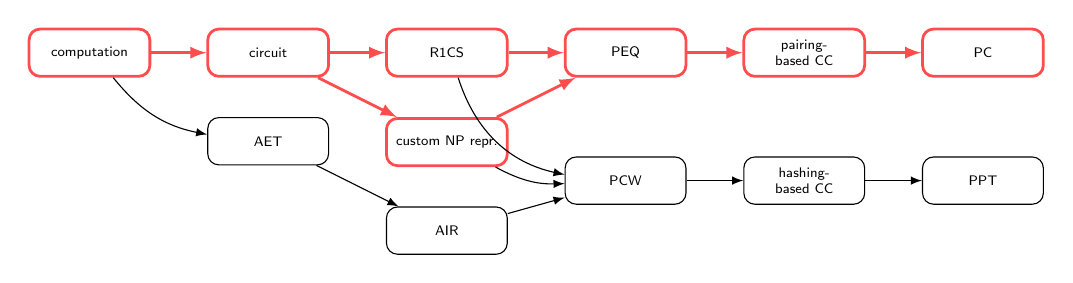
\begin{tikzpicture}[
        node distance=0.8cm,
        box/.style={rectangle, draw, rounded corners, minimum width=1.4cm, minimum height=0.6cm, text width=1.3cm, align=center, font=\tiny},
        box-highlight/.style={rectangle, draw=red!70, line width=1pt, rounded corners, minimum width=1.4cm, minimum height=0.6cm, text width=1.3cm, align=center, font=\tiny},
        arrow/.style={->, >=latex, font=\tiny},
        arrow-highlight/.style={->, >=latex, draw=red!70, line width=1pt, font=\tiny}
    ]

    % Define nodes - first column
    \node[box-highlight] (comp) {computation};

    % Second column
    \node[box-highlight] (circ) [right=0.7cm of comp] {circuit};
    \node[box] (aet) [below=0.5cm of circ] {AET};

    % Third column
    \node[box-highlight] (r1cs) [right=0.7cm of circ] {R1CS};
    \node[box-highlight] (cust) [below=0.5cm of r1cs] {custom NP repr.};
    \node[box] (air) [below=0.5cm of cust] {AIR};

    % Fourth column
    \node[box-highlight] (polyid) [right=0.7cm of r1cs] {PEQ};
    \node[box] (cw) [below=1cm of polyid] {PCW};

    % Fifth column
    \node[box-highlight] (crypto) [right=0.7cm of polyid] {pairing-based CC};
    \node[box] (crypto2) [below=1cm of crypto] {hashing-based CC};

    % Sixth column
    \node[box-highlight] (pair) [right=0.7cm of crypto] {PC};
    \node[box] (prox) [below=1cm of pair] {PPT};

    % Define connections
    \draw[arrow-highlight] (comp) -- (circ);
    \draw[arrow] (comp) to[bend right=20] (aet);

    \draw[arrow-highlight] (circ) -- (r1cs);
    \draw[arrow-highlight] (circ) -- (cust);
    \draw[arrow] (aet) -- (air);

    \draw[arrow-highlight] (r1cs) -- (polyid);
    \draw[arrow-highlight] (cust) -- (polyid);
    \draw[arrow] (air) -- (cw);
    \draw[arrow] (cust) to[bend right=15] (cw);
    \draw[arrow] (r1cs) to[bend right=30] (cw);

    \draw[arrow-highlight] (polyid) -- (crypto);
    \draw[arrow] (cw) -- (crypto2);

    \draw[arrow-highlight] (crypto) -- (pair);
    \draw[arrow] (crypto2) -- (prox);

    \end{tikzpicture}
    \caption{A general workflow describing how SNARKs reduce checking computation to checking polynomials. The highlighted path shows the course pairing-based approaches take. Acronyms: AET = algebraic execution trace, AIR = algebraic intermediate representation, CC = cryptographic compilation, PCW = polynomial codeword, PEQ = polynomial equality, PC = pairing check, PPT = polynomial proximity testing, R1CS = rank-1 constraint system.}
    \label{fig:snark-workflow}
\end{figure}
\noindent Modern SNARKs largely use the "workflow" depicted in figure \ref{fig:snark-workflow} to prove/verify computation. Here there are two courses; one reduces to checking polynomial relationships using pairing-based cryptography (left), and the other reduces to checking proximity to a Reed-Solomon code via combination of coding theoretic results and merkle trees. In an interactive setting, the "checks" or "testing" steps might involve randomized interaction with the verifier; but many interactive-proof-based methods use Fiat-Shamir to have the prover simulate such interaction, which the verifier can check. To balance coverage, depth, and accessibility, this paper focuses on approaches involving pairing-based cryptography (highlighted paths). We leave the surveying of methods using hashing-based cryptography as future work, but we note that like pairing-based methods, their effectiveness stems from how the NP computation being verified is represented.

\subsection{Representing the complexity class NP}
\noindent How SNARKs `'frame' the computation to verify directly influences how synergistic each method is with algebraic objects like polynomials and the cryptographic methods applied to them. This in turn affects the proof size and prover/verifier complexity, all of which are highly relevant to blockchain infrastructure/applications using SNARKs. Clearly, one must use an NP-complete language compatible with other aspects of the method in question. The most immediate choice of representation is boolean circuit satisfiability; in light of the use of polynomials, a reasonable sequel is \textit{arithmetic} circuit satisfiability, in which the circuit of importance uses addition gates in place of OR gates, and multiplication gates in place of AND gates. Wires can also take on values in some prime field $F_p$  rather than just 0 or 1. Another reasonable step forward is via more direct polynomial representations of NP discussed below.

\begin{definition}[Rank-1 Constraint System (R1CS)]\label{def:r1cs}
\noindent Let $m, n \in \mathbb{N}$. A rank-1 constraint system (R1CS) consists of the matrices $L, R, O \in \mathbb{F}_{p}^{m \times (n+1)}$. A vector $w \in \mathbb{F}_p^{n+1}$ with $w_0 = 1$ satisfies the R1CS if:
\begin{align}
    Ow = (Lw) \circ (Rw)
\end{align}
\noindent where $\circ$ denotes the Hadamard (element-wise) product.
\end{definition}

\noindent Here, the second dimension is increased to account for constant values in the constraint system. We now loosely describe how to reduce an instance of arithmetic circuit-SAT to R1CS-SAT. First, preprocess the arithmetic circuit so that addition gates become sums of values along multiplication gate input wires. Then, one can view row $i$ of $L$ as a ``selector row'' for the values in $w$ that, when linearly combined via row $L_i$, form the left input to multiplication gate $i$. The same logic applies for $R$ and $O$. Populating $L, R, O$ accordingly yields the above relationship between three matrix-vector products -- in other words, three rank-1 matrices (hence ``rank-1''). In some sense, this consolidates the equations in the constraint system used by Bootle et al. \cite{bootlezkargs}, which uses two separate equations for multiplication gate constraints and linear constraints. It is also reducible to yet another important representation of NP based on polynomial equality checking, defined below.

\begin{definition}[Regular Quadratic Arithmetic Program (QAP)]\label{def:qap}
\noindent Let $m, n \in \mathbb{N}$. A regular Quadratic Arithmetic Program $Q$ over a field $\mathbb{F}_p$ consists of the following:
\begin{itemize}
    \item The target polynomial $t(x) = \prod_{i=1}^m (x - i)$
    \item The polynomials $\{u_i(x), v_i(x), w_i(x)\}_{i=0}^n$ % , where $u_i(j) = L_{ji}$, $v_i(j) = R_{ji}$, and $w_i(j) = O_{ji}$
\end{itemize}

\noindent A vector $c = (c_0 \dots c_n) \in \mathbb{F}_p^{n+1}$ with $c_0 = 1$ satisfies the QAP $Q$ if and only if there exists a polynomial $h(x)$ such that:
\begin{align}
    p(x) = \left(\sum_{i=0}^n c_i u_i(x)\right) \cdot \left(\sum_{i=0}^n c_i v_i(x)\right) - \left(\sum_{i=0}^n c_i w_i(x)\right) = h(x)t(x) = 0 \mod t(x)
\end{align}
\end{definition}

\noindent Again, we loosely describe one reduction from arithmetic circuit-SAT to regular QAP-SAT. First preprocess the gate as described before. Then label each of the multiplication gates $1$ through $m$. Then reduce to R1CS-SAT as described before. Now, define $t(x)$ as mentioned, which forms the polynomial that vanishes whenever $x \in \{1 \dots m\}$ (is a gate identifier). Then for $j \in \{0 \dots n\}$ define each $u_j(x), v_j(x), w_j(x)$ such that $u_j(i) = L_{ij}, v_j(i) = R_{ij}, w_j(i) = O_{ij}$ for all $i \in \{1 \dots m\}$. Evaluating $p(i)$ then effectively checks whether the constraint for gate $i$ is satisfied using the defined $u_j(x), v_j(x), w_j(x)$. In other words, it evaluates $(L_i \cdot c) (R_i \cdot c) - (O_i \cdot c)$, which should be zero for a satisfying assignment and nonzero otherwise. The polynomials include a constant term ($j = 0$), and we typically set $c_0 = 1$ to enable constants in the polynomials analogous to the R1CS-SAT instance. The constants involved in the gates represented by the R1CS-SAT instance would be in the ``0th column'' of each matrix.\\

\noindent Though not exhaustive by any means, these two representations of NP already yield a a connection between the computation being verified, arithmetic circuit satisfiability, and an instance of polynomial equality/divisibility checking. From this point, the polynomial check can be verified in a hidden fashion using pairing-based cryptography. This idea is used by virtually all pairing-based methods, with modifications to the constraint system and the polynomial relationship being checked.

\subsection{Polynomial Distinguishability}
\noindent As mentioned, modern SNARKs reduce proving/verifying statements about computation to polynomial identity/property testing via suitable characterizations of NP. The use of polynomials over other mathematical objects is justified by how little information one needs to distinguish between two polynomials, which is a consequence of the following lemma.

\begin{lemma}{Schwarz-Zippel lemma}
\noindent Let $f(x_1, x_2, \dots x_n) \in R[x_1 \dots x_n]$ be a nonzero polynomial in $n$ variables defined over an integral domain $\mathbb{F}^{n}$. Suppose the element $(a_1, a_2, \dots a_n)$ is selected uniformly at random from a finite subset $S \subset \mathbb{F}^n$. Then 
$$
    \Pr(f(a_1, a_2, \dots a_n) = 0) \le \frac{\text{deg}(f)}{|S|}
$$
\end{lemma}

\noindent where $\text{deg}(f)$ is the maximum sum of the degrees of any term's variables. It immediately follows that if $f = g-h$, then for a randomly sampled point $(a_1, \dots a_n) \in \mathbb{F}$, we have that $\Pr(g(a_1, \dots a_n) = h(a_1, \dots a_n))$ is bounded from above by $\frac{d}{|\mathbb{F}|}$. In other words, $g$ and $h$ will output different values at $(a_1 \dots a_n)$ with high probability if they are not equal, assuming the $d$ and $\mathbb{F}$ are chosen so that $d \ll |\mathbb{F}|$. Thus, given the right choice of degree and field size, a verifier will still be able to distinguish between two unequal polynomials with high probability using a single evaluation point. Succinct argument systems can make use of this to check polynomial equalities at a single point, enjoying small proof size and little probability of spurious equality.

\subsection{Pairing-based Cryptography}
\noindent Pairing-based cryptography \cite{ibepairings} allows one to check algebraic relationships between quantities ``in the exponent'' using bilinear functions on arbitrary source group elements (usually from elliptic curve groups). This technique works well with checking polynomial equalities and is frequently used in modern SNARKs as a result.  This paper abstracts elliptic curve groups and pairings for brevity; we instead focus on the properties they exhibit which make pairing-based cryptography useful in this setting.\\

\noindent Suppose we have two cyclic elliptic curve groups $\mathbb{G}_1$ and $\mathbb{G}_2$ generated by elements $G_1$ and $G_2$, respectively. We denote the scalar multiple of a point $P \in \mathbb{G}_i$ by $kP$, which is just the same as $k$ additions of $P$ and $k \in \mathbb{F}_s$ where $\mathbb{F}_s$ is the scalar field determining the scalars one can multiply points in $\mathbb{G}_1, \mathbb{G}_2$ by. For a bilinear pairing $e: \mathbb{G}_1 \times \mathbb{G}_2 \to \mathbb{G}_t$ where $P_1 \in \mathbb{G}_1$ and $P_2 \in \mathbb{G}_2$, we have the following properties:
\begin{itemize}
    \item for $a, b \in \mathbb{F}$, $e(aP_1, bP_2) = e(P_1, P_2)^{ab}$
    \item for $Q_1 \in \mathbb{G}_1$, $e(P_1+Q_1, P_2) = e(P_1, P_2) e(Q_1, P_2)$
    \item for $Q_2 \in \mathbb{G}_2$, $e(P_1, P_2+Q_2) = e(P_1, P_2) e(P_1, Q_2)$
    \item $e(G_1, G_2)$ generates $\mathbb{G}_t$ (non-degeneracy)
\end{itemize}

These properties make it easy to check multiplicative relationships. For instance, suppose we have three polynomials $A(x), B(x), C(x)$ and we want to check that $A(\alpha)B(\alpha) = C(\alpha)$ for some input $\alpha$. From bilinearity of $e$ it follows that 
\begin{align*}
e(G_1, G_2)^{A(\alpha)B(\alpha)} &= e(G_1, G_2)^{C(\alpha)} \\
\Leftrightarrow e([A(\alpha)]_1, [B(\alpha)]_2) &= e([C(\alpha)]_1, G_2)
\end{align*}
where $[A(\alpha)]_1 = A(\alpha)G_1$ (same idea for the other values). So if we can reduce checking circuit satisfiability to checking a polynomial equality at a point, we can send elliptic curve points as proof elements with which the verifier would perform such a pairing check. 

\subsection{Polynomial commitment schemes (PCS)}
\noindent A polynomial commitment scheme is a protocol by which a prover claims they know a polynomial $f(x)$ satisfying some relationship, and a verifier checks this claim. A noteworthy example of such a relationship is that $f(y) = z$ for some fixed $y, z$. We detail a noteworthy polynomial commitment scheme for this exact task known as the Kate-Zaverucha-Goldberg commitment scheme (KZG) \cite{kzg}. Suppose $P$ wants to prove they know $f$ of degree $d$ such that $f(\beta) = z$. It follows that $f(X) - z$ is divisible by $(X - \beta)$, so we should be able to construct $h(X) = \frac{f(X) - z}{X - \beta}$ since we know $f$. $P$ commits to $f$ and $h$ by their hidden evaluations on some $\alpha$ agreed upon in advance by the $P$ and the verifier $V$. In practice, the evaluations are hidden via scalar multiplication by an elliptic curve group generator $g_1 \in \mathbb{G}_1$. This scheme uses two elliptic curve groups for this purpose, so assume the point $g_2$ generates the EC group $\mathbb{G}_2$. Let $[a]_i = ag_i \in \mathbb{G}_i$. Suppose $\mathcal{P}$ and $\mathcal{V}$ agree on a \textit{trusted setup} containing the hidden terms $\{[1]_1, [\alpha]_1, [\alpha^2]_1, \dots [\alpha^{d}]_1, [1]_2, [\alpha]_2\}$. $P$ sends $[f(\alpha)]_1$ and $[h(\alpha)]_2$. $V$ then sends a challenge point $\gamma$ to which $\mathcal{P}$ responds with $[f(\gamma)]_1$ and $[h(\gamma)]_1$. $V$ then checks that $f(\gamma) - z = h(\gamma)(\gamma - \alpha)$ where $h$ was constructed from the evaluation requirement we wanted to prove that $f$ satisfies. For a bilinear pairing function $e : \mathbb{G}_1 \times \mathbb{G}_2 \to \mathbb{G}_t$, $\mathcal{V}$ checks that 
\begin{align}
&e([f(\gamma) - z]_1, g_2) = e([h(\gamma)]_1, [\gamma]_2 - [\alpha]_2) \\
&\Leftrightarrow e(g_1, g_2)^{f(\gamma) - z} = e(g_1, g_2)^{h(\gamma)(\gamma - \alpha)} \\
&\Leftrightarrow  f(\gamma) - z = h(\gamma)(\gamma - \alpha)
\end{align}

\noindent KZG commitment schemes require constant size communication since the polynomials involved can be collapsed to a point without losing virtually any distinguishability. Given their use of elliptic curve groups to meet this end, their security depends on the hardness of computing elliptic curve discrete logarithms (find $\alpha$ given the points $g$ and $\alpha g$), for which no classical polynomial time algorithm is known \cite{ecdlp}. The drawbacks of using this scheme include the need to generate a trusted setup and the lack of post-quantum security. Being quite customizable, KZG works with batching, multivariate polynomials, and various optimizations for faster polynomial operations. That said, many methods use different polynomial commitment schemes, some of which avoid pairing-based cryptography entirely. Nonetheless we opt for this example to give an idea of commitment schemes making use of pairings, as this is relevant to many modern pairing-based SNARKs.
%Elliptic curve groups are preferred here due to small key sizes, which are determined by the size of the base field the point coordinates are from. There is also a group operation over elliptic curve points behaving like addition, in which one computes a sum of points $A + B$ by reflecting over the $x$-axis the point on both the curve and the line $AB$ (if $A = B$ we use the tangent line through $A$). We can then define multiplication of a point $A$ by some $s \in \mathbb{F}_s$ in the curve's \textit{scalar field} as summing $s$ copies of $A$. Here, $s$ can be considered an \textit{elliptic curve discrete logarithm} and is believed to be hard to compute given $A$ and $sA$; this is the elliptic curve variant of the discrete log assumption. The hardness of this problem yields a scheme for additively homomorphic encryption: given a cyclic multiplicative group $\mathbb{G}$ over some wisely-chosen elliptic curve and its generator $G$, encrypt $x$ as $xG \in \mathbb{G}$. Pairings are defined to behave like multiplication (linear in each input), enabling a way to take the ``product'' of hidden terms.

\section{Circuit-specific pairing-based SNARKs}
\subsection{The QAP recipe}
\noindent The seminal PCP theorem results \cite{pcpthm1, pcpthm2} yielded a powerful characterization of NP as a set of languages with polynomial-time PCP verifiers only needing to check a constant number of proof bits \textit{regardless of statement size}. However, early work on pairing-based SNARKs by Gennaro et al. \cite{snarknopcp} was motivated by the possibility of succinct arguments of knowledge using a representation \textit{more suitable} than PCPs for integration with cryptographic primitives. To this end, Gennaro et al. \cite{snarknopcp} coined quadratic span programs (QSP) and quadratic arithmetic programs (QAP). These representations of NP allow one to reduce checking a computation to checking a multiplicative relationship between two polynomials in a way that ``computes'' the circuit representing the computation. Although the QSP construction is noteworthy, we limit discussion to their QAP-related construction due to the clearer connection to arithmetic circuits and downstream polynomial checking. We recall the strong QAP form here:
\begin{align}
\underbrace{\left(\sum_{j=1}^n a_i v_i(x)\right)}_{\text{left inputs}} \cdot \underbrace{\left(\sum_{j=1}^n b_i w_i(x)\right)}_{\text{right inputs}} - \underbrace{\left(\sum_{j=1}^n c_i y_i(x)\right)}_{\text{outputs}} = h(x) t(x) \equiv 0 \mod t(x)
\end{align}

\noindent This representation is compiled into cryptographic proof elements via an additively homomorphic encoding $E$ -- namely, a one-to-one function for which addition operations are preserved in the output space, and inversion is difficult. Given an instance of arithmetic circuit satisfiability one is trying to prove/verify, $E$ serves to compile the corresponding QSP/QAP instance checking polynomial divisibility (by $t(x)$) into a proof containing just 9 group elements (non-ZK). We detail the non-zero-knowledge version here for clarity, denoting $E(x)$ by $[x]$. The prover $\mathcal{P}$ computes the quotient polynomial $h(x)$ and sends
\begin{align*}
    \pi = \Big(&[v_{mid}(s)], [w(s)], [y(s)], [h(s)], \\ 
    &[\alpha v_{mid}(s)], [\alpha w(s)], [\alpha y(s)], [\alpha h(s)], \\ 
    &[\beta_v v_{mid}(s) + \beta_w w(s) + \beta_y y(s)]\Big)
\end{align*}

where $\alpha, s, \beta_v, \beta_w, \beta_y \in \mathbb{F}_p, $ are secret random preprocessing elements; $v_{mid}(s), w(s), y(s)$ are the witness-weighted combinations of the wiring polynomials in the QAP; and $h(s)$ is the evaluation of the quotient polynomial an honest prover would know. In particular, $v_{mid}(x) = \sum_{k \in \mathcal{I}_{mid}} a_k v_k(x)$ where $\mathcal{I}_{mid}$ are the indices corresponding to private circuit inputs. $w(x), y(x)$ are defined similarly, but over all $k \in \{0 \dots m\}$. The verifier in turn checks 5 equations using the additive properties of $E$. In particular, the verifier receives the following proof $\pi'$ \textit{which it does not yet know is valid}, hence the new notation of elements reminiscent of those in $\pi$:
\begin{align*}
\pi' = (\pi_{v_{mid}}, \pi_{w}, \pi_{y}, \pi_{h}, \pi_{v'_{mid}}, \pi_{w'}, \pi_{y'}, \pi_{h'}, \pi_{z'})
\end{align*}

\noindent $\mathcal{V}$ then checks 6 pairing equations involving the components of $\pi'$ (recall the pairing notation from earlier section):  
\begin{align}
&e([v_0(s) + v_{in}(s) + v_{mid}(s)]_1, [w_0(s) + w_{in}(s) + w_{mid}(s)]_2) = \\ 
&e([t(s)]_1, [h(s)]_2) \cdot e([y_0(s) + y_{in}(s) + y_{mid}(s)]_1, G_2) \\
&e([v_{mid}'(s)]_1, G_2) = e([v_{mid}(s)]_1, [\alpha]_2) \\
&e([w'(s)]_1, G_2) = e([w(s)]_1, [\alpha]_2) \\
&e([y'(s)]_1, G_2) = e([y(s)]_1, [\alpha]_2) \\
&e([h'(s)]_1, G_2) = e([h(s)]_1, [\alpha]_2) \\
&e([z'(s)]_1, [\gamma]_2) = e([\beta_v v_{mid}(s) + \beta_w w(s) + \beta_y y(s)]_1, [\gamma]_2)
\end{align}
\noindent where $v'_{mid}(s)$ is encoded in $\pi_{v'_{mid}}$, $w'(s)$ is encoded in $\pi_{w'}$, and so on. The first one checks the QAP divisibility relation. The next four equations are based on knowledge-of-exponent assumptions; they check if $\mathcal{P}$ knows the wiring polynomials used in the proof. The last equation checks that $\mathcal{P}$'s proof used wiring polynomials consistent with those agreed upon in the trusted setup. \\


\subsection{More optimized QAP-based methods}
\noindent GGPR uses a \textit{strong} QAP for their scheme, which uses a different set of coefficients for each sum in the QAP equation. This mandates a \textit{strengthening step} in which extra constraints between the coefficient sets are materialized, tripling prover work and preprocessing size. Parno et al. \cite{pinocchio} made the simple optimization of using a \textit{regular} QAP, which uses the same set of coefficients $a_i$ for each sum in the QAP expression, contrary to the $a_i, b_i, c_i$ seen in the strong QAP form. This change eliminated the need for the strengthening step without any noteworthy compromises, although it required modifications to proof elements and verification checks that ensure consistent use of coefficients in QAP terms. Another improvement was the use of an asymmetric pairing operation $e: \mathbb{G}_1 \times \mathbb{G}_2 \to \mathbb{G}_t$ such that $\mathbb{G}_1 \ne \mathbb{G}_2$, which in practice is 3-4x as efficient as its symmetric counterpart $(\mathbb{G}_1 = \mathbb{G}_2)$. Imaginably, both of these optimizations appear in the following QAP-based approaches.\\

\noindent With these two methods (among others) as a springboard, Groth \cite{groth16} used stronger security assumptions to optimize proof size, setup size, and verifier complexity. Groth still used the regular QAP representation; but unlike previous methods that compiled each polynomial evaluation into two group elements, he compiled the wiring polynomials to just one (ex. just $w(s)$ instead of $w(s), \alpha w(s)$). Combined with some algebraic manipulation, this eliminated multiple setup terms, reduced proof size to 3 group elements, and reduced verifier operations to a single pairing check using three pairings. However, this single-element compilation prevents use of knowledge-of-exponent assumptions, so security is argued in the generic group model (GGM) \cite{ggmlower} where, loosely speaking, adversaries cannot exploit group specific properties or encodings of group elements. While seemingly strong, such assumptions are not necessarily uncalled for, as Gentry et al. showed that SNARKs for NP languages cannot exist without strong -- namely, non-falsifiable -- assumptions to begin with \cite{nonfalsifiable}. Reduction in proof size and verifier complexity could also be regarded as "worth it" on this front. Possessing zero-knowledge properties in addition to these other traits, Groth's work (colloquially known as groth16) unsurprisingly saw large adoption in blockchain systems verifying privacy-preserving homogeneous computation. Applications like Tornado Cash \cite{tornadocash} use this method to verify withdrawals from privacy-preserving pools without exposing source-destination address relationships; and UTXO-based privacy-preserving blockchains like Zerocash network \cite{zcash} used groth16 to prove/verify presence of unspent funds in the Merkle tree inherent to the UTXO model. 
\begin{table}[!t]
\caption{Comparison of work done by pairing-based SNARKs. 
$n$ represents the number of circuit gates; $\mathbb{G}_1$ and 
$\mathbb{G}_2$ represent group elements; $\mathbb{F}$ represents field elements; $\mathbf{P}$ represents pairing operations. 
In prover/verifier work columns, $\mathbb{G}_i$ and $\mathbb{F}$ refer to elliptic curve group scalar multliplications in $\mathbb{G}_i$ 
and field element multiplications in $\mathbb{F}$, respectively. An asterisk implies the method is not fully succinct. Where more fine-grained 
source group information is easily discerned, $\mathbb{G}$ implies the elements / operations could be in either source group.
Where more fine-grained information is not available or easily comparable in a standardized manner, we resort to asymptotic terms.}
\label{tbl:snark}
\begin{tabular}{|l|l|l|p{3.2cm}|l|c|c|l|}
\hline
\toprule
method & CRS size & $\mathcal{P}$ work (asymp.) & proof size & $\mathcal{V}$ work & universal & updatable & assumptions \\ \hline\toprule
\midrule
GGPR13 & $O(n) \mathbb{G}$ & $O(n) \mathbb{G}$ & $9 \mathbb{G}$ & $14 \mathbf{P}$ & No & No & q-PKE, q-PDH \\ \hline
PGHR13 & $O(n) \mathbb{G}$ & $O(n) \mathbb{G}$ & $8 \mathbb{G}$ & $11 \mathbf{P}$ & No & No & $q$-PKE, $q$-PDH \\ \hline
Groth16 & $9n \mathbb{G}_1, 3n \mathbb{G}_2$ & $n \mathbb{G}_1$ & $2 \mathbb{G}_1, 1 \mathbb{G}_2$ & $3 \mathbf{P}$ & No & No & $q$-type, GGM \\ \hline
GMKL18 & $O(n^2) \mathbb{G}$ & $O(n) \mathbb{G}_1$ & $2 \mathbb{G}_1, 1 \mathbb{G}_2$ & $5 \mathbf{P}$ & Yes & Yes & $q$-type, KOE \\ \hline
MBKM19 & $36n \mathbb{G}_1$ & $273n \mathbb{G}_1$ & $20 \mathbb{G}_1, 16 \mathbb{F}$ & $13 \mathbf{P}$ & Yes & Yes & AGM \\ \hline
Gab19* & $2n \mathbb{G}_1$ & $8n \mathbb{G}_1$ & $6 \mathbb{G}_1, 4 \mathbb{F}$ & $5 \mathbf{P}$ & Yes & Yes & AGM \\ \hline
GWC19 & $3n \mathbb{G}_1, 2 \mathbb{G}_2$ & $11n \mathbb{G}_1$ & $7 \mathbb{G}_1, 6 \mathbb{F}$ & $2 \mathbf{P}, 16 \mathbb{G}_1$ & Yes & Yes & AGM \\ \hline
GW21 & $9n \mathbb{G}_1, 2 \mathbb{G}_2$ & $35n \mathbb{G}_1$ & $4 \mathbb{G}_1, 15 \mathbb{F}$ & $5 \mathbb{G}_1, 2 \mathbf{P}$ & Yes & Yes & AGM \\ \hline
CHM+19 & $(4n +2) \mathbb{G}_1$ & $22n \mathbb{G}_1$ & $13 \mathbb{G}_1, 8 \mathbb{F}$ & $2 \mathbf{P}$ & Yes & Yes & AGM \\ \hline\bottomrule
\bottomrule
\bottomrule
\end{tabular}
\end{table}

% \begin{align}
% \underbrace{\left(\sum_{j=1}^n a_i v_i(x)\right)}_{\text{left inputs}} \cdot \underbrace{\left(\sum_{j=1}^n a_i w_i(x)\right)}_{\text{right inputs}} - \underbrace{\left(\sum_{j=1}^n a_i y_i(x)\right)}_{\text{outputs}} = h(x) t(x) \equiv 0 \mod t(x)
% \end{align}
% \begin{align}
% r_v, r_w, s, \alpha_v, \alpha_w, \alpha_y, \beta, \gamma &\overset{R}\leftarrow \mathbb{F} \\
% r_y &= r_v r_w \\
% g_v &= r_v G \\
% g_w &= r_w G \\
% g_y &= r_y G
% \end{align}

% \noindent The prover $\mathcal{P}$ would send 
% \begin{align}
%     \pi_2 = \Big(&[v_{mid}(s)], [w_{mid}(s)], [y_{mid}(s)], [h(s)], \\
%     [&\alpha_v v_{mid}(s)], [\alpha_w w_{mid}(s)], [\alpha_y y_{mid}(s)], \\
%     [&\beta_v v_{mid}(s) + \beta_w w_{mid}(s) + \beta_y y_{mid}(s)]\Big)
% \end{align}

% \noindent where like before, $v_{mid}(x) = \sum_{k \in \mathcal{I}_{mid}} a_k v_k(x)$ and likewise for $w_{mid}(x)$, $y_{mid}(x)$. Similar to GGPR, the verifier receives
% $$
% \textbf{THE POTENTIALLY VALID PROOF THE VERIIFER RECEIVES}
% $$
% and checks the following pairing-based equations:
% \begin{align}
% e([v_0(s) + v_{in}(s) + v_{mid}(s)]_1 \cdot [w_0(s) + w_{in}(s) + w_{mid}(s)]_1, G_2) = \\
% ([t(s)]_1, [h(s)]_2) \cdot e([y_0(s) + y_{in}(s) + y_{mid}(s)]_1, G_2) \\
% e([r_v v'_{mid}(s)], G) = e([v_{mid}(s)], [r_v \alpha]) \\
% e([r_w w'_{mid}(s)], G) = e([w_{mid}(s)], [r_w \alpha]) \\
% e([r_y y'_{mid}(s)], G) = e([y_{mid}(s)], [r_y \alpha]) \\
% e(z'(s), [\gamma]) = e([r_v v_{mid}(s) + r_w w_{mid}(s) + r_y y_{mid}(s)], [\beta \gamma])
% \end{align}

\section{Circuit-independent (universal) pairing-based SNARKs}
\noindent Homogeneous computation aside, circuit-specific pairing-based methods have a couple of noteworthy shortcomings. The first of these as noted by Groth \cite{grothupdatable} is that there is no way of ensuring the deployers of the SNARK in question have disposed of the secret randomness used to generate the trusted setup. The second and more important issue is a lack of flexibility due to the use of computation-dependent (non-universal) preprocessing. As an example, we depict the groth16 trusted setup here. As in the QAP definition, the $u_i(x), v_i(x), w_i(x)$ encode the contribution of the $i$-th witness component to left input, right input, and output of gate $x$ respectively. 
\begin{align}
\sigma = \Big( 
    &[\alpha]_1, [\beta]_1, [\gamma]_1, [\delta]_1, \{[x^i]_1\}_{i \in [0, n-1]}, \{[\gamma^{-1}(\beta u_i(x) + \alpha v_i(x) + w_i(x))]_1\}_{i \in [0, \ell]}, \\
    &\{[\delta^{-1}(\beta u_i(x) + \alpha v_i(x) + w_i(x))]_1\}_{i \in [\ell+1, m]}, \\
    &\{[\delta^{-1} x^i t(x)]_1\}_{i \in [0, \deg(h)]}, [\beta]_2, [\gamma]_2, [\delta]_2, \{[x^i]_2\}_{i \in [0, n-1]}
\Big)
\end{align}

\noindent As is the case with other discussed methods, the contributions of the $i$-th witness component to gate $x$ are ``stuck'' in the encrypted $u_i(x), v_i(x), w_i(x)$ (not the component's value, but its index). Thus if the circuit wiring changes, these polynomials must change to reflect this. Updating the setup incrementally, however, is not possible for two reasons, either of which is sufficiently limiting. The first is the hidden $u_i(x), v_i(x), w_i(x)$ are interpolated from relationships between witness components and the gates they feed into. Adding a new gate and its associated wire connections would require adding a new data point to each of these polynomials. Thus, one would have to re-interpolate all of them which is not possible without violating cryptographic assumptions (since they are encrypted) or regenerating the entire setup, which defeats the purpose of updates. Another related reason concerns the setup's combination of these hidden polynomial terms, such as the $[\beta u_i(x) + \alpha v_i(x) + w_i(x)]_1$. Groth \cite{grothupdatable} showed these setup terms could be used to extract the the constituent monomials and ultimately break soundness if the setup allowed updates. These observations suggest that the conception of a QAP-based updatable SNARK is unlikely, and that different approaches are necessary. Such approaches should be \textit{universal}, in the sense that they allow proving computation of any structure up to a certain size; and \textit{updatable}, meaning that the trusted setup can be efficiently updated by any party and remains sound if at least one setup contributor is honest. This idea becomes highly relevant when deploying blockchain systems using SNARKs with trusted setups. After one update to the setup (which can be performed by anyone with a corresponding proof), users do not have to worry about the network being subverted by its deployers or other adversaries. As they stray from the QAP-based paradigm which seems to be ``maxed out'', the following methods use a more diverse set of arithmetizations and polynomial checking to fulfill these universality/updatability related goals.\\

\noindent To this end, Groth \cite{grothupdatable} produced a universal and updatable scheme using a multivariate polynomial encoding of QAP elements. Although this scheme had constantn proof size, constant verification complexity, and a linear-time procedure by which a linear-size circuit-specific setup could be produced as needed, true universality required quadratically many terms w.r.t circuit size. Furthermore, SRS updates would take a quadratic number of group exponentiations and update verification a linear number of pairing operations. For circuits with millions of gates this is impractical. However, this attempt hints that a SNARK with linear-size universal \& efficiently updatable setup could be attainable if the setup terms are univariate (and monomial). Maller et al. achieved this with Sonic, which draws inspiration from techniques of Bootle et al. \cite{bootlezkargs} reducing circuit satisfiability to checking Laurent polynomials encoding a Hadamard matrix product (models mul. gate operations) paired with a linear constraint system (models wire connections \& addition gates). They also use a permutation argument inspired by Bootle et al. \cite{grothshuffle} to enforce correct copying of values across linked wires. The setup contains only univariate monomials and therefore requires linear space, though it is twice the space one would like due to the presence of $X^{-i}$ term for every $X^i$ term (loosely written). Being composed of monomials, the setup can be updated by any party supplying a corresponding proof of update validity. In a realistic deployment of this scheme, the setup would not be circuit dependent, and a single update could eliminate the risk that the deployers still hold valid setup secrets.\\ 

\noindent Though significant in its own right, Sonic suffers from two shortcomings. First, it is not fully verifier-succinct. Second and foremost, there are large constants in the proof construction complexity. A likely cause is the attempt to accommodate for $n$-fan-in circuits whose gates can accept arbitrarily many inputs. While a reasonable generalization, this allows any given linear constraint the ability to use arbitrarily many witness inputs, requiring the use of entire witness and selector vectors for each constraint. It also causes a bloated permutation argument since a given gate may require arbitrarily many copy constraints between its own inputs and outputs from preceding gates that feed into it. Gabizon et al. \cite{plonk} addressed these issues with a simplifying assumption that may not catch one's eye, but turns out to have important performance implications: simply let each circuit gate take two inputs. The impact of this is twofold. Firstly, it enables a much simpler constraint representation of arithmetic circuit-SAT, where for an $n$ gate circuit we have the following constraint for gate $i$. Here $a_i, b_i, c_i$ the indices in $\mathbf{x}$ corresponding to the left input, right input, and output of the $i$-th gate, respectively; and $\mathbf{q_L}, \mathbf{q_R},\mathbf{q_O},\mathbf{q_M},\mathbf{q_C},$ are ``selector vectors'' determining which gate-related values partake in the constraint. This allows one to express addition or multiplication gates in the same constraint by setting $(\mathbf{q_L})_i, (\mathbf{q_R})_i, (\mathbf{q_M})_i$ accordingly. 
\begin{align}
(\mathbf{q_L})_i \cdot \mathbf{x}_{(\mathbf{a})_i} + (\mathbf{q_R})_i \cdot \mathbf{x}_{(\mathbf{b})_i} + (\mathbf{q_O})_i \cdot \mathbf{x}_{(\mathbf{c})_i} + (\mathbf{q_M})_i \cdot (\mathbf{x}_{(\mathbf{a})_i} \cdot \mathbf{x}_{(\mathbf{b})_i}) + (\mathbf{q_C})_i = 0
\end{align}

    % &\Leftrightarrow \textbf{q}_{a} \circ \textbf{a} + \textbf{q}_{b} \circ \textbf{b} + \textbf{q}_{M} \circ (\textbf{a} \circ \textbf{b}) + \textbf{q}_{C} \circ \textbf{c} = \textbf{0}

\noindent During proof construction, these terms are collected into polynomials $q_L(x), a(x), q_R(x), b(X),$ etc. and combined in the same manner as the original constraint equation. Secondly, the 2-fan-in assumption enables optimizations to the permutation argument inspired by Groth et al. and Maller et al. \cite{grothshuffle, sonic}. While sonic used a product check accounting for the arbitrarily many copy constraints per gate, each product check per gate involves three terms in the numerator and denominator each, resulting in a ``grand product'' used in proof construction. We show the non-zero-knowledge version here, but adding ZK properties requires shifting this equation by adding a ``masking'' polynomial that still vanishes on the desired domain in order to not corrupt the expression.
\begin{align}
    z(X) &= L_1(X) + \\
    &\sum_{i=1}^{n-1} L_{i+1}(X) \prod_{j=1}^{i} \frac{(w_j + \beta\omega^j + \gamma)(w_{n+j} + \beta k_1\omega^j + \gamma)(w_{2n+j} + \beta k_2\omega^j + \gamma)}{(w_j + \beta\sigma^*(j) + \gamma)(w_{n+j} + \beta\sigma^*(n+j) + \gamma)(w_{2n+j} + \beta\sigma^*(2n+j) + \gamma)}
\end{align}

\noindent where $L_i(x) = \frac{X^n - 1}{X - \omega^i}$ is the $i$-th Lagrange basis polynomial defined over the $n$-th roots of unity (gives 1 when $X = \omega^i$ and 0 otherwise). Notably, the polynomial check works well with a common optimization to PlonK's invocation of KZG scheme; by representing the hidden monomials in the Lagrange basis, the point evaluations of polynomials can be computed in $O(d)$ operations where $d$ is the degree of the polynomial in question, which is faster than the $O(d \log d)$ complexity for interpolation via inverse FFT \& subsequent evaluation. The pairing check performed by the verifiere is also ``fixed argument'' in the second source group, enabling both of only 2 pairings the verifier performs to be 30\% faster than the traditional pairing \cite{fapairings}.\\

\noindent The combination of flexibility, intuitive arithmetization, and better efficiency has made PlonK a gateway to other methods increasing expressiveness and performance, with important implications for so-called ``zero-knowledge virtual machines'' (zkVMs). Ambrona et al. \cite{turboplonk} proposed methods to optimize the constraint system used, as well as optimized circuits for PlonK-based verifiable implementations of the ``SNARK-friendly'' Poseidon hash function \cite{poseidon}. For zkVM operations less compatible with SNARK systems, Gabizon et al. proposed Plookup \cite{plookup} which adapts the PlonK permutation argument to verify that a set of values is present in some predetermined table; this is particularly useful for constraining the correctness of zkVM operations involving nonlinear operations that would make the resulting circuits / constraint system inefficient to verify. A notable example is a ``SNARK-unfriendly'' hash function like SHA-3 \cite{sha3}, which has many nonlinear bit-mixing operations. Variations like halo2 \cite{halo2} and plonky2 \cite{plonky2} combine the PlonK arithmetization with commitment schemes inspired by Bulletproofs \cite{bulletproofs} and FRI \cite{fri} respectively to shed the need for a trusted setup at the expense of slower verification. These two advancements highlight the customizability of the PlonK system, which is futher explored among other methods in the following sections.

% Chiesa et al. improved upon this with Marlin \cite{marlin}, a more verifier-succinct approach which cryptographically compiles a ``sparsity-friendly'' polynomial representation of an R1CS instance for the verifier to check algebraic consistency of via pairings. Within, both methods make use of bi-variate and univariate KZG commitments, respectively; more importantly, they also make use of \textit{permutation arguments}, which prove the correct copying of values in consecutive circuit wires. As a key occurrence of flexibility-performance tradeoff, the latter sub-argument is necessary due to the encoding of witness-gate relationshiphs directly in the proof instead of the setup.\\

\section{Applications}

\begin{figure}[!t]
\centering
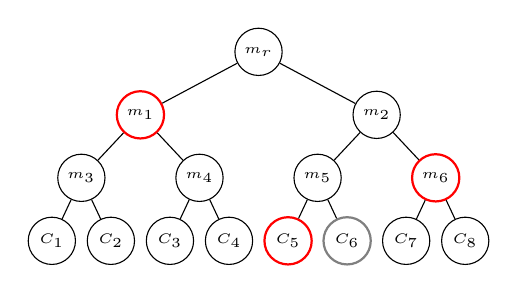
\begin{tikzpicture}[
    level 1/.style={sibling distance=30mm, level distance=8mm},
    level 2/.style={sibling distance=15mm, level distance=8mm},
    level 3/.style={sibling distance=7.5mm, level distance=8mm},
    every node/.style={draw, circle, minimum size=6mm, inner sep=0pt, font=\tiny}
]
    % Root node
    \node {$m_r$}
        % Level 1
        child {node[draw=red, line width=0.8pt] {$m_1$}
            % Level 2
            child {node {$m_3$}
                % Level 3
                child {node {$C_1$}}
                child {node {$C_2$}}
            }
            child {node {$m_4$}
                % Level 3
                child {node {$C_3$}}
                child {node {$C_4$}}
            }
        }
        child {node {$m_2$}
            % Level 2
            child {node {$m_5$}
                % Level 3
                child {node[draw=red, line width=0.8pt] {$C_5$}}
                child {node[draw=gray, line width=0.8pt] {$C_6$}}
            }
            child {node[draw=red, line width=0.8pt] {$m_6$}
                % Level 3
                child {node {$C_7$}}
                child {node {$C_8$}}
            }
        };
\end{tikzpicture}
\caption{Merkle tree with authentication path (in red) for deposit commitment $C_6$ (in gray) used by applications like Tornado cash. Here, $C_6$ is recursively hashed with its children all the way to the root. If the computed root matches $m_r$ at deposit time, then the user is allowed to withdraw the amount of funds specified in $C_6$.}
\label{fig:merkle-tree}
\end{figure}

\subsection{Application/Infrastructure-Level Privacy Preservation}
\noindent Traditional blockchain network innerworkings expose transaction details, making privacy preservation nontrivial at the application/infrastructure layers. Applications like Tornado Cash \cite{tornadocash} partially solve this problem at the application layer, using groth16 proofs to enable privacy-preserving deposits and withdrawals to different wallets without revealing the link between the two. Withdrawing funds involves proving membership of one's deposit record in a Merkle tree, as shown in figure \ref{fig:merkle-tree}; combined with tight EVM smart contract gas limits, the homogeneous nature of this computation makes groth16 a suitable choice. Blockchains like Zerocash \cite{zcash} (privacy-preserving version of Bitcoin \cite{bitcoin}) somewhwat generalize tornado cash's abilities using the unspent transaction output (UTXO) model, where spending funds requires proving knowledge of an ``unspent funds'' record in a Merkle tree. Early versions of Zerocash used groth16 for this, but the NU5 upgrade of 2022 switched to the universal halo2 proof system \cite{halo2}, which enables a combination of a PlonK-style arithmetization and Bulletproofs-style commitment scheme \cite{bulletproofs} requiring no trusted setup at the expense of verifier performance. Beyond such homogeneous computation, non-universal (zk)SNARKs could be used for application-specific privacy-preserving blockchains as well (ex. a blockchain for private trading/lending). 

\subsection{zkVMs and ``Layer-2'' Scaling Solutions for Ethereum Network}
\noindent Layer-2 (L2) blockchains \cite{l2survey} have emerged as a dominant scaling solution to layer-1 (L1) chains like Ethereum \cite{ethereum}. These alternate blockchains are essentially Ethereum forks with their own application layer and transaction processing; however, they settle batches of transactions directly on Ethereum network. These alternate outlets afford users a similar experience while easing computational load on the Ethereum chain. ``Zero-knowledge'' virtual machines (zkVMs) \cite{scrollzkevm, polygonzkevm, sp1, risc0, openvm} are a crucial component of this architecture, as they produce succinct proofs of L2 block validity which are later settled by verifier contracts on the L1 chain. zkVMs using PlonK variants \cite{scrollzkevm} have already played a huge role in the functionality of zkVMs powering widely used L2 chains \cite{scrollarch}. Further advancements in lookup arguments based on either PlonK or other methods will have huge impacts on transaction processing speed, layer 2 network performance, and ultimately the scalability of Ethereum network itself.  

% \noindent A crucial point of consideration here is that not all computations performed in VVMs are ``SNARK-friendly''; a prime example of this is hash functions like SHA256 which use non-linear or non-algebraic operations like bit mixing. This can cause the circuits constraining this computation to be overly complex and inefficient. To meet this end, lookup-based methods are of great interest here since they can avoid constraining ``SNARK-unfriendly'' operations directly without losing soundness. An example of this is lies in the proof for validity of transaction that called a contract function using \texttt{sha256()}. Instead of constraining the exact sha-256 computation, the prover and verifier would agree on a publicly known table of acceptable inputs and outputs for SHA-256, which the prover commits to as part of the proof. The verifier does not need to know the whole table - they just need to know a commitment to the one considered correct. This can then be compared with what the prover committed to.\\

\section{Future Research}

\subsection{Post-quantum algebraically-friendly SNARKs}
\noindent Though multiple of the SNARKs discussed are practical from a performance standpoint, quantum computers may render them useless from a security standpoint in the near future. As a result, there is a strong effort to develop efficient enough post-quantum SNARKs. To this end, many works \cite{starks, ligero, fractal, spartan, jolt} use hashing-based based Reed-Solomon proximity testing methods \cite{fri}, which relies on the hardness of computing hash function collisions. While such approaches are believed to be post-quantum secure, the cryptographic primitives used offer no additively homomorphic structure enabling the recursive composition of smaller proof elements \& faster verification we see in pairing-based methods. Albrecht et al. \cite{lattice1} made some progress in this direction via a lattice-based SNARK with logarithmic-time verification; it derives security from the hardness of the short integer solution (SIS) problem in lattices. Future work that quantifies the security assumptions in this area and decreases prover/verifier complexity could realize practical SNARKs using additively homomorphic post-quantum encryption, which the blockchain ecosystem would eventually accept given sufficient tooling and support.

\subsection{Automated verification of SNARK methods/applications}
\noindent Currently, several layer 2 blockchains collectively hold tens of billions of dollars \cite{l2beat} protected by the integrity of SNARK methods used to verify block validity; if either the methods or their implementations have soundness bugs, it could allow a knowledgeable adversary to prove an invalid state transition for financial gain, causing massive financial loss to users and the chain. There are two noteworthy and related directions of ongoing work in this domain. The first is related to formally verifying the SNARK methods themselves in various mechanized cryptographic models using Lean 4 \cite{arklib, lean4} and other techniques for lookup-based arguments, as done with JOLT zkVM \cite{jolt, joltfv}. Though very promising and easily updatable, there are still many gaps to fill. Furthermore, the periodic introduction of new methods will require constant updates to the relevant types and theorems. Nonetheless, seeking formal guarantees on SNARK behavior in various mechanized theoretical models will make them increasingly fit for use in large-scale DeFi infrastructure/applications needing to verify computation. A more adversarial direction concerns automated detection of missing circuit constraints \cite{picus}, which detect nondeterministic circuit behavior using symbolic execution and SMT solvers. Picus has been used heavily in verifying Risc Zero VM \cite{risc0} Preliminary work by Chaliasos et al. \cite{sok} has found that circuit-related soundness bugs are the most frequent kind of bug by a huge margin, suggesting that building upon this existing work will be important for the security of VVMs. For instance, it would be extremely useful to have tools detect missing constraints in circuits validating interacting sub-witnesses like in the STARK-based SP1 zkVM architecture, which uses LogUp \cite{logup} to verify correctness of interactions.

% \subsection{Integration of optimizations to pairing-based cryptography}
% \noindent optimize miller function\\
%
% \subsection{Standardized benchmarks for pairing-based methods (and others)}
% \noindent Current SNARK benchmarks lack standardization by the computation being verified.\\


% \subsection{Proof aggregation \& Distributed Proving}
% \noindent As one would expect, proof generation remains the performance bottleneck in most SNARKs (pairing-based or not). In a world where computational resources are quite asymmetrically distributed (DeFi being no exception), it would be sensible to be able to outsource more intensive computations within the same proof to another party; naturally they would include a proof that such computation was done correctly. \textbf{Is there any work on this right now}. A similar idea emerges when we consider distributed proving of a statement by segmenting the \textit{statement} instead of the \textit{proof components}. Each delegated prover would then have to prove that a given subcircuit has an assignment which produces some desired value, then all of these proofs would get aggregated along with a proof that the aggregation was performed correctly.\\
%
%
% \subsection{Extending pairings to higher-degree operations}
% \noindent nothing\\


\newpage
\ifnum\fullversion=0
  \bibliographystyle{splncs03}
 \else
   \bibliographystyle{alpha-short}
 \fi
\bibliography{cryptobib/abbrev3,cryptobib/crypto,add}

\end{document} 
